\documentclass[11pt,a5paper]{article}

% --- Packages ---
\usepackage{times}          % Times font
\usepackage[left=1.5cm,right=1.5cm,top=1.5cm,bottom=1.5cm]{geometry}
\usepackage{setspace}       % For line spacing
\usepackage{titlesec}       % Title formatting
\usepackage{indentfirst}    % Indent first paragraph
\usepackage{ragged2e}       % For justified text
\usepackage{graphicx}
\usepackage{subcaption}
\usepackage{caption}
\usepackage{float}
\usepackage{enumitem}
\pagestyle{empty}
\setlength{\parindent}{0.51cm} % Indent for new paragraphs

% --- Custom title format ---
\newcommand{\papertitle}[1]{%
    \begin{center}
        {\fontsize{14}{16}\selectfont \textbf{#1}\par}
    \end{center}
}

\newcommand{\paperauthor}[2]{%
    \begin{center}
        {\fontsize{11}{13}\selectfont #1, #2\par}
    \end{center}
}

\newcommand{\paperyearroll}[2]{%
    \begin{center}
        {\fontsize{11}{13}\selectfont #1, #2\par}
    \end{center}
}

% --- Begin Document ---
\begin{document}
\singlespacing

% Title
\papertitle{Reduced Graphene Oxide (rGO) based
Conductometric Sensors for Drinkable Water
Quality Monitoring}

% Author
\paperauthor{Soham Kanti Payra}{IRPE}
\vspace{-2em}
% Year and Roll Number
\paperyearroll{4th year}{Roll Number: T91/ECE/224085}

\justifying
\vspace{-1.5em}
\section{Introduction}
Access to clean drinking water is essential, but current monitoring systems are often expensive and technically complex. 
This project aimed to develop a low-cost, scalable sensor using reduced graphene oxide ($rGO$) and molybdenum disulfide 
($MoS_{2}$) to detect heavy metal ions in water.

The proposed sensor leverages the high conductivity of $rGO$ and the semiconducting nature and surface activity 
of $MoS_{2}$. 
A heterojunction formed by these materials enhances sensitivity and enables effective signal transduction 
upon analyte interaction.


\vspace{-1.5em}
\section{Materials and Fabrication}
Synthesis of $rGO$ and $MoS_{2}$:
\vspace{-0.5em}
\begin{itemize}[itemsep=0pt]
    \item Graphene Oxide (GO) was synthesized using the modified Hummer’s method,
    involving the oxidation of graphite using $KMnO_{4}$ and $H_{2}SO_{4}$ under carefully controlled temperatures. 
    \item $MoS_{2}$ nanosheets were produced using liquid-phase exfoliation in aqueous ammonia. 
    Ultrasonication at 5°C for 3 hours ensured effective exfoliation while preserving structural quality.
\end{itemize}

Device Fabrication:
The sensor was constructed using sequential drop-casting- 7 layers of rGO drop-casted 
on a clean glass substrate and dried at $70^{\circ}C$, with a Teflon tape mask applied to define the junction region,
and 3 layers of $MoS_{2}$ dispersion deposited on the unmasked area to form the receptor layer.

\vspace{-1.5em}
\section{Characterization and Results}
Structural and Morphological Characterization:
\vspace{-0.5em}
\begin{itemize}[itemsep=0pt]
    \item X-ray diffraction (XRD) confirmed that GO was successfully reduced to $rGO$ (peak near 24–26°).
    $MoS_{2}$ showed characteristic peaks around 14.4°, indicating layered structure.
    \item FESEM (Field Emission Scanning Electron Microscopy) revealed $rGO$ nanoflakes with uniform film formation, and
    $MoS_{2}$ nanosheets evenly distributed, confirming good adhesion and structure.
\end{itemize}

Electrical Characterization:
A 4-point probe cryogenic station showed that the device displayed Shottky-type I-V characteristics,
confirming the formation of a p–n heterojunction, which is crucial for sensing functionality.

\begin{figure}[t]
    \centering
    % First Row
    \begin{subfigure}[b]{0.325\textwidth}
        \centering
        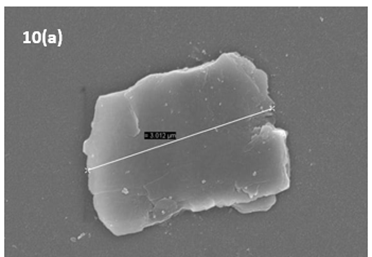
\includegraphics[width=\linewidth]{fesem_rGO.png}
        \caption{FEESEM of $rGO$}
    \end{subfigure}
    \hfill
    \begin{subfigure}[b]{0.325\textwidth}
        \centering
        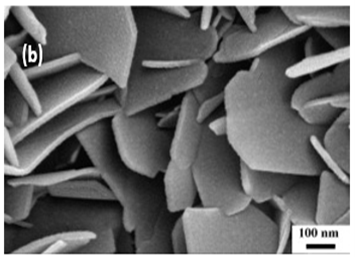
\includegraphics[width=\linewidth]{fesem_MoS2.png}
        \caption{FESEM of $MoS_{2}$}
    \end{subfigure}
    \hfill
    \begin{subfigure}[b]{0.325\textwidth}
        \centering
        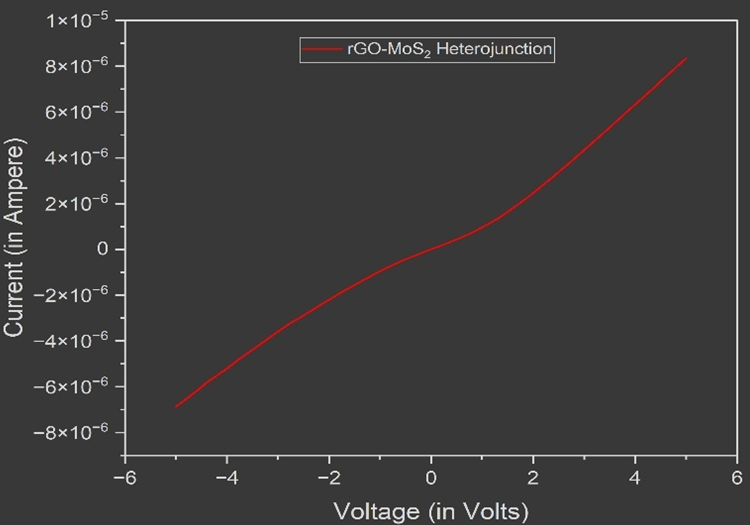
\includegraphics[width=\linewidth]{elec_char.png}
        \caption{XRD of the sensor}
    \end{subfigure}

    \vspace{0.5cm}

    % Second Row
    \begin{subfigure}[b]{0.325\textwidth}
        \centering
        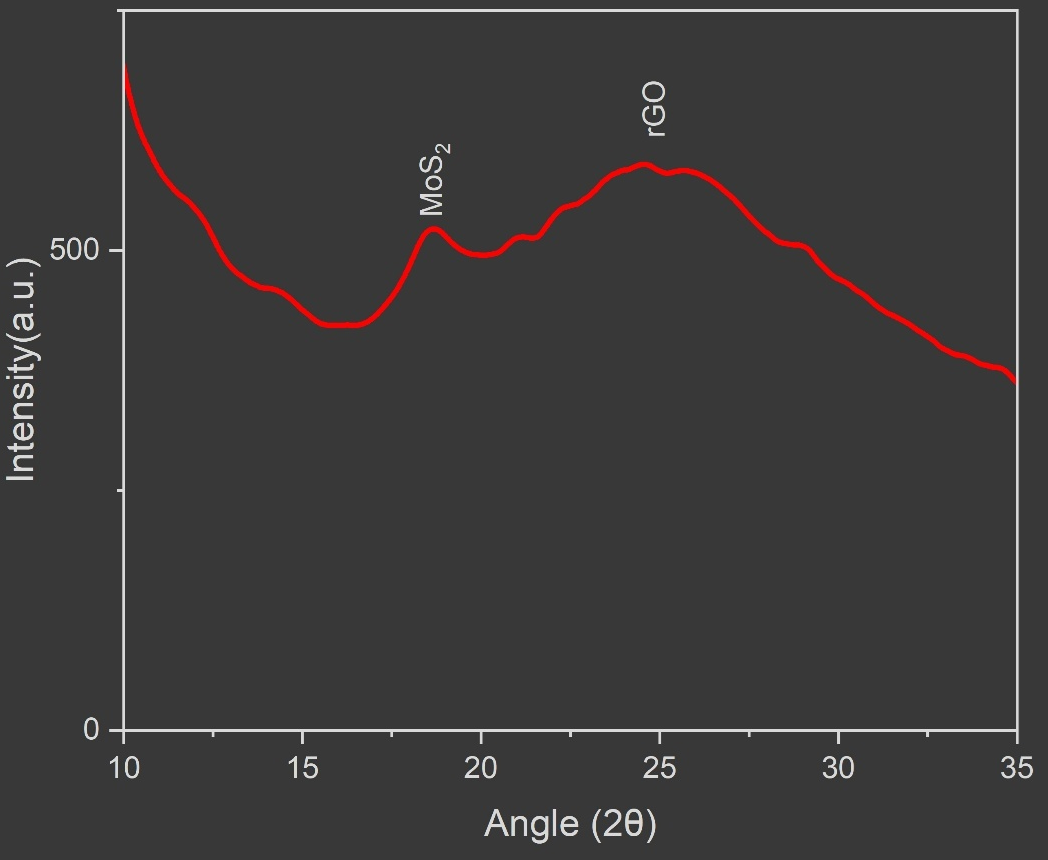
\includegraphics[width=\linewidth]{xrd.png}
        \caption{I-V characteristic}
    \end{subfigure}
    \hfill
    \begin{subfigure}[b]{0.325\textwidth}
        \centering
        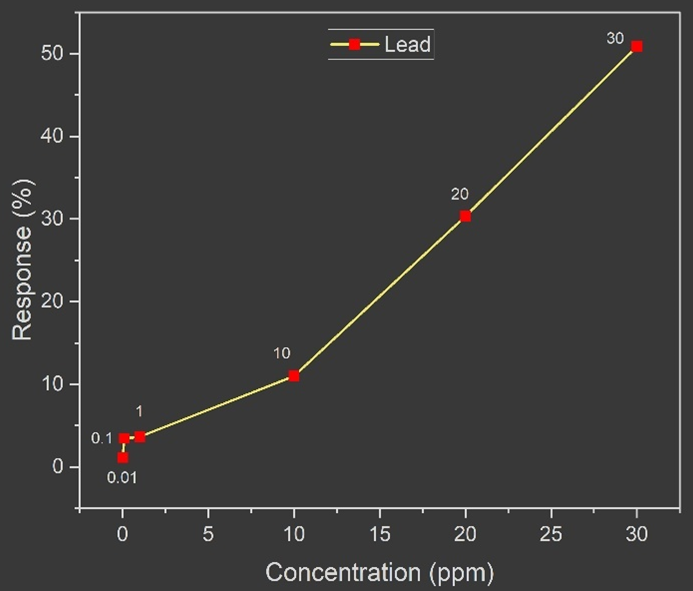
\includegraphics[width=\linewidth]{lead_ion.png}
        \caption{Response to $Pb^{2+}$}
    \end{subfigure}
    \hfill
    \begin{subfigure}[b]{0.325\textwidth}
        \centering
        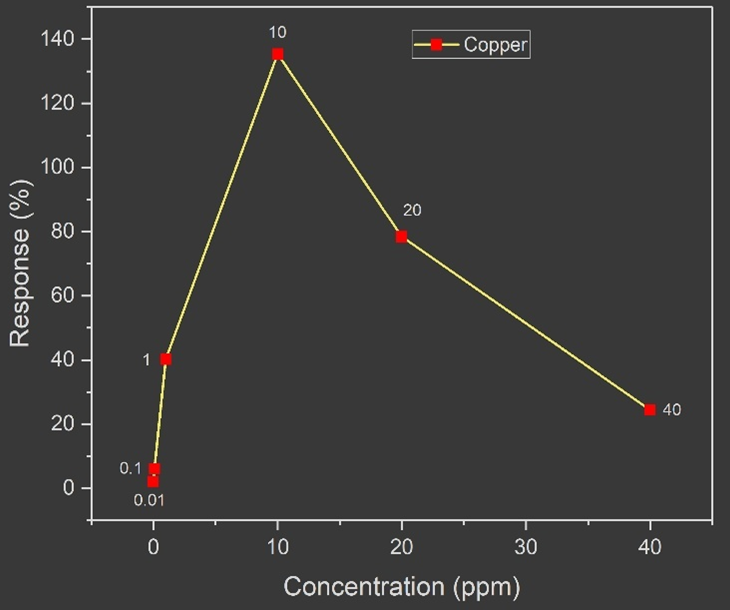
\includegraphics[width=\linewidth]{copper_ion.png}
        \caption{Response to coppper}
    \end{subfigure}
    \caption{Results}
    \label{fig:results}
\end{figure}

\vspace{-1.5em}
\section{Conclusion}
The sensor was tested with five heavy metal ions: 
Nickel, Cadmium, Mercury, Lead, and Copper, across multiple concentrations.
\begin{itemize}
    \item Highest selectivity and sensitivity observed for $Pb^{2+}$ (Lead ions).
    \item Copper ions also showed strong response at higher concentrations.
    \item Sensor performance for $Pb^{2+}$ was both quantifiable and consistent, with response $>50\%$ at 30 ppm.
\end{itemize}

\end{document}